\section{Methodology}
\epigraph{\RaggedLeft``It doesn't stop becoming magic just because you know how it works.''}{\textit{Sir Terry Pratchett}\\\textit{Discworld, 1983}}

\subsection{Overview}
\begin{figure}[H]
	\centering
	\tikzstyle{block} = [rectangle, draw, fill=blue!20, text centered, rounded corners, minimum height=2em, align=center]
	\tikzstyle{block2} = [rectangle, draw, fill=green!20, text centered, rounded corners, minimum height=2em, align=center,
	text width=3.5cm]
	\tikzstyle{line} = [draw, -latex]
	\usetikzlibrary{positioning}
	
	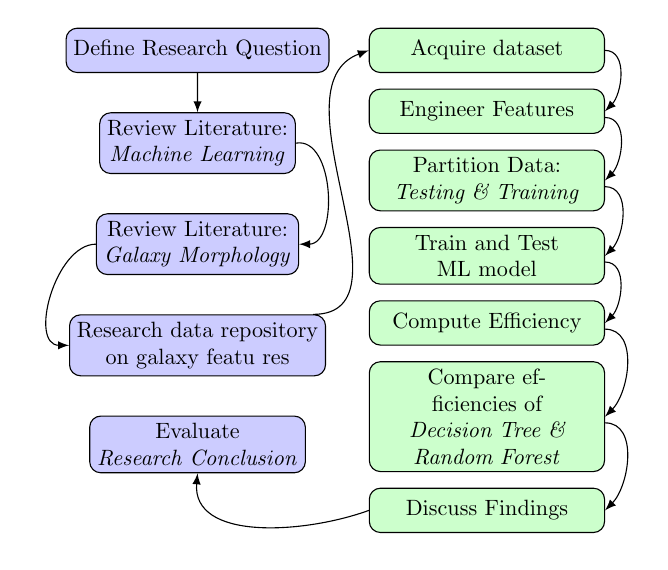
\begin{tikzpicture}[node distance=.5, scale=0.8, every node/.style={scale=0.8}]	
		\node[block] (drq) {Define Research Question};
		\node[block, below=of drq] (rl){Review Literature:\\\emph{Machine Learning}};
		\node[block, below=of rl]  (rl2){Review Literature:\\\emph{Galaxy Morphology}};
		\node[block, below=of rl2] (rpd){Research data repository\\on galaxy featu res};
		\node[block2, right=of drq] (ad) {Acquire dataset};
		\node[block2, below= .2cm of ad ](ef) {Engineer Features};
		\node[block2, below=.2cm of ef] (pt) {Partition Data:\\\emph{Testing \& Training}};
		\node[block2, below=.2cm of pt] (trm) {Train and Test ML model};
		\node[block2, below=.2cm of trm] (ce) {Compute Efficiency};
		\node[block2, below=.2cm of ce] (ced) {Compare efficiencies of\\\emph{Decision Tree \& Random Forest}};
		\node[block2, below=.2cm of ced] (dr) {Discuss Findings};
		\node[block, below=of rpd] (er) {Evaluate\\\emph{Research Conclusion}};
		
		\path[line] (drq) -- (rl);
		\path(rl.east) edge[line, out=10,in=0] (rl2.east);
		\path(rl2.west) edge[line, out=180,in=-180] (rpd.west);
		\path(rpd.15) edge[line, out=0,in=200] (ad.west);
		\path (ad.east)  edge[line, out=0,in=45] (ef.east);
		\path (ef.-3)  edge[line, out=0,in=45]  (pt.east);
		\path (pt.-3)  edge[line, out=0,in=45]  (trm.east);
		\path (trm.-3)  edge[line, out=0,in=45]  (ce.east);
		\path (ce.-3)  edge[line, out=0,in=45]  (ced.east);
		\path (ced.-3)  edge[line, out=0,in=45]  (dr.east);
		\path (dr.west)  edge[line, out=200,in=-95]  (er.south);
	\end{tikzpicture}
	\caption{Research Methodology that I have followed.}
	\label{fig:rm}
\end{figure}

\subsection{Regression Classifiers}
Before exploring the classification, a decision tree is first applied to the regression problem. The following sections deal with the determination of redshifts of galaxies from their photometric colours. It is independent of the morphological classification of galaxy however the flux data of both the problems are shared by the galaxy. Hence the same data can be used to predict both redshift and morphology. Although the colour profiles across 5 SDSS\footnote{The SDSS is one of the longest-running astronomical observation that scans the multi-spectral redshifts of galactic matter. It employs a 2.5m wide-angle telescope housed at the Apache Point Observatory in New Mexico, USA \parencite{sloan_digital_sky_survey_sloan_2014}} filters\footnote{Light is the goldmine of information used by astronomers to, deduce for example a star or a galaxy's distance, composition, mass, temperature and other attributes. And colours are the functions of different wavelength of light. Here, to predict the type of galaxy one of the feature is colour. Astronomers have precisely defined colour to accommodate all its complexities devoid of any subjectivity. Colour is the difference of luminous flux/brightness of source between two filters. SDSS uses 5 filters - u(ultra-violet), g(green), r(ed), i(near-infrared), and z(infrared). Infrareds are invisible to the human eye. A galaxy with high g-r (difference) colour is redder than one with low g-r colour.} Thus flux data across 5 bands are one of the most significant features in this project. are present in both the problems. I have deliberately included the regression problem before tackling the morphological classification in order to demonstrate how decision tree can work for both classifications and for regression problems and to complement classification with the learnings from regression. Moreover, the difference in terms of the way the efficiency of the decision tree is assessed in each case is also significant.

\subsubsection{Photometric Redshift}
Since time immemorial, the night sky has evoked wonder in the heart of man and his mind has ever since been restless to discern the mysteries of the universe. The existential questions of origin have intrigued philosophers and cosmologists exchanging insights into the nature of the universe. Surpassing the steady-state model, modern cosmology has now discovered multiple independent verifications (such as the cosmic microwave background radiation) for the beginning of the universe \parencite{ross_why_2008}.  The standard model now sets the age of the universe at approximately 13.7 billion, whence it was born in a cataclysmic event known as the Big Bang. Since then the universe has ever been expanding.

\paragraph{Galaxy Redshift \& Big Bang} One of the earliest determiners for the expanding universe is the result of Edwin Hubble's meticulous observations of galaxies. In 1929, Hubble proved that distant galaxies exhibited Doppler effect as their optical spectra showed a redshift in the emitted light \parencite*{hubble_relation_1929}. This was a clear indication that galaxies were moving away from the point of sight and in-fact every cosmic object was flying apart as the space between them stretched. If one were to rewind the cosmic movie of expanding universe, then there would come a point when everything would collapse back at a singular point known as the singularity which is the boundary of space, time, matter, and energy \parencite[18]{davies_god_2007}.

Redshift is a significant phenomenon in astronomy that proved the expanding universe. In the presence of spectral fingerprint of elements in the earth that are also found in galaxies, it is quite straightforward to calculate the redshift of the galaxy. The redshift is obtained by subtracting the elemental spectrograph data into the observed galaxy's spectrograph data. an example is shown in figure \ref{fig:rsp}. However, the process can be time-consuming and tedious for large samples. Likewise, without the reference and when the only spectrum for the galaxy is available it can be difficult to estimate the photometric shifts. This is where machine learning can help. Given the accurately calculated spectrum for other galaxies, the ML model is able to predict the redshifts in new galaxies.

\begin{figure}[H]
	\centering
	\includegraphics[width=\linewidth,keepaspectratio]{images/misc/plot_sdss_filters_2.png}
	\caption{SDSS Filters, Reference Spectrum, and Redshifting Spectrum(ref image sdss).}
	\label{fig:rsp}
\end{figure}

\subsubsection{Magnitudes and Colours}
The features used in the training dataset comprises of the flux magnitudes of the Sloan Digital Sky Survey (SDSS) catalogue to create the colour index. The flux magnitude is the intensity of light or total light received in five frequency bands - u, g, r, i, and v through the SDSS filters.

\subsubsection{Decision Trees in Python}
In this prediction, the decision colour indices from photometric imaging will be the input and the photometric redshift will be the output. In the decision tree, the colour indices are the features at the top nodes and the target label - the redshift value which is continuous is reaches the leaf nodes at the bottom. This is depicted in the tree shown in figure \ref{fig:tree}
\begin{figure}[H]
	\centering
	\includegraphics[width=\linewidth,keepaspectratio]{images/misc/d.png}
	\caption{Graphic view of decision tree generated in Python for the redshift regression.}
	\label{fig:tree}
\end{figure}

The python machine learning library \inlinecode{Python}{scikit-learn} is used as the regression classifier. I take in the input features along with the corresponding target values, then constructs a tree model that it employs to predict new data.

\subsubsection{The Sloan Data}
The Sloan data is a \inlinecode{Python}{NumPy} object which is a structured array. The \inlinecode{Python}{NumPy} package in Python is a fundamental tool for scientific computing. It provides features such as powerful multi-dimensional array with useful manipulation functions (). The colour indices and redshift data is stored as shown in table \ref{tbl:tbn}

\begin{table}[ht]
	\centering
	\begin{tabular}{rrrrrrr}
		u & g & r & i & z & ... & redshift\\
		\hline
		19.84 &    19.53 &    19.47 &    19.18 &    19.11 &    ... & 0.54\\
		19.86 &    18.66 &    17.84 &    17.39 &    17.14 &    ...    & 0.16\\
		...    & ... &    ... & ... &    ... &...\\
		18.00 &    17.81 &    17.77 &    17.73 &    17.73 &    ...    & 0.47
	\end{tabular}
	\caption{ A sample of content in the NumPy record - Flux magnitudes across 5 colour indices with redshift value.}
	\label{tbl:tbn}
\end{table}
The ellipsis in between hints at additional data and also the presence of columns 'spec\_class' and 'redshift\_err' which is not required in this case. 

\subsubsection{Features \& Targets}
Extraction of features and target definition is written in the function\\ \inlinecode{Python}{get_features_targets} shown in figure \ref{fig:gft0}
\begin{figure}[H]
	\centering
	\frame{\includegraphics[width=.6\linewidth,keepaspectratio]{images/code/features_targ.png}}
	\caption{Subroutine to extract features and to define the target.}
	\label{fig:gft0}
\end{figure}
It splits the training data into input features and the respective targets. In this case, the 4 colour indices and the respective redshifts as targets. It returns a tuple of:
\begin{itemize}
	\item \textbf{features}: a \inlinecode{Python}{NumPy} array of n by 4 dimensions, where n is the number of galaxies or the dataset size.
	\item \textbf{targets}: a 1-dimensional \inlinecode{Python}{NumPy} array of size n, containing the corresponding redshift value for each galaxy.
\end{itemize}

Specific columns can be accessed with the index name. For example, the `z' flux magnitude and its redshift can be accessed as\\ \inlinecode{Python}{data['u']} and \inlinecode{Python}{data['redshift']}respectively. The four features are the colour difference `u-g',`g-r',`r-i',i-that have been dynamically calculated from existing columns.

\subsubsection{Limitations of Non-ML approach}
The redshift prediction based on colour index could be approached by a non-machine-learning approach. An empirical model could be constructed to predict the change in redshift value (dependent variable) with uni or multi-variate colour indices (independent variable).
\begin{figure}[H]
	\centering
	\includegraphics[width=\linewidth,keepaspectratio]{images/misc/redshift-U-G.png}
	\caption{Redshift vs Colour index `u-g'.}
	\label{fig:rvc}
\end{figure}
For example, in the graph above a non-linear regression function could be constructed. Least mean squares could be used to determine the best fit. It can be predicted from the spread of values that this model would be a complex one such as an inverse sine function. The model obtained could be used. However, it would turn out to be highly complex and there would be no assurance that it would yield reliable results. 
\begin{figure}[H]
	\centering
	\includegraphics[width=\linewidth,keepaspectratio]{images/misc/redshift-colour-colour.png}
	\caption{Redshift vs two colour indices.}
	\label{fig:rvi}
\end{figure}
Another approach could be to graph colour-index vs colour-index plot using the additional bands to depict the redshift. An example of this is shown above in figure \ref{fig:rvi}. The two indices show certain defined regions where redshifts are similar. A combination of other indices could be used and plotted on a contour map. However, the resulting redshift estimates would have significant uncertainties.

\subsubsection{Decision Tree Regressor}
The readied features and targets needs to fed to the decision tree model so that it can learn before making the predictions. The \inlinecode{Python}{DecisionTreeRegressor} class from \inlinecode{Python}{sklearn.tree} is used for this. The algorithm is initialised by the statement\\ \inlinecode{Python}{drt=DecisionTreeRegressor()}. To train the model, we use the \inlinecode{Python}{fit} method while passing the parameters \inlinecode{Python}{features} and \inlinecode{Python}{targets} as: \inlinecode{Python}{dtr.fit(features, targets)}. The \inlinecode{Python}{dtr} object now trained can be used to make the prediction. This is achieved by the statement:\\ \inlinecode{Python}{predictions=dtr.predict(features)}. Here, \inlinecode{Python}{predictions} is an array of predicted redshift values mapping to each of the galaxy. The first 4 predictions are seen below in figure \ref{fig:prr}
\begin{figure}[H]
	\centering
	\frame{\includegraphics[width=.7\linewidth,keepaspectratio]{images/code/pred_reg.png}}
	\caption{Method - Decision Tree Regression Prediction.}
	\label{fig:prr}
\end{figure}
The output is the first 4 predictions is seen below in figure \ref{fig:prro}:
\begin{figure}[H]
	\centering        \frame{\includegraphics[width=\linewidth,keepaspectratio]{images/code/pred_reg_o.png}}
	\caption{First 4 predictions of redshifts.}
	\label{fig:prro}
\end{figure}

\subsubsection{Evaluating The Accuracy}
\begin{figure}[H]
	\centering
	\frame{\includegraphics[width=.8\linewidth,keepaspectratio]{images/code/accuracy_reg.png}}
	\caption{Code to calculate the accuracy using the median difference.}
	\label{fig:acr}
\end{figure}
To ensure the accurate prediction in regression, the predictions generated by the model and the actual values are compared to test the accuracy of the model and thus its performance. The difference between the actual and predicted value is the residual. It can give a preliminary assessment of the model's performance. There are multiple methods for residual \parencite{liitiainen_residual_2009}, where the median of differences of predicted and actual value is used. It is calculated as:
\begin{align*}
	A&=M(|Y_{i,predicted} - Y_{i_actual}|)\\
	\text{where}~A &= \text{accuracy,}\\
	M&=\text{median,}\\
	||&=\text{absolute value of the difference}
\end{align*}
To achieve the median difference in code, the following method shown in figure \ref{fig:med}is prepared:
\begin{figure}[H]
	\centering
	\frame{\includegraphics[width=.8\linewidth,keepaspectratio]{images/code/accuracy_reg.png}}
	\caption{Subroutine to compute the median difference.}
	\label{fig:med}
\end{figure}
\subsubsection{Hold-out Validation}
The decision tree regression shown above used the common dataset for both training and testing the decision tree. This is only the optimisation of the model to get the best results for only training data. Hence, it does not provide a realistic estimate for accuracy for unseen galaxies. The way to solve the problem is to split the dataset into two subsets - training and testing. This method of validation is known as the hold-out method \parencite{schneider_cross_2019}. The corresponding python \inlinecode{Python}{method validate_model} which receives model, features, and targets as input arguments, is shown below in figure \ref{fig:hov}
\begin{figure}[H]
	\centering
	\frame{\includegraphics[width=.8\linewidth,keepaspectratio]{images/code/accuracy_reg.png}}
	\caption{Subroutine for hold-out validation.}
	\label{fig:hov}
\end{figure}
Hold-out validation method invocation is shown below in figure \ref{fig:hvc}. And the output is shown in figure \ref{fig:hvo}
\begin{figure}[H]
	\centering
	\frame{\includegraphics[width=.8\linewidth,keepaspectratio]{images/code/hov_call.png}}
	\caption{Hold-out validation method invocation}
	\label{fig:hvc}
\end{figure}
\begin{figure}[H]
	\centering
	\frame{\includegraphics[width=\linewidth,keepaspectratio]{images/code/hov_call_o.png}}
	\caption{Median difference after Hold-out validation.}
	\label{fig:hvo}
\end{figure}
As shown in figure \ref{fig:hvo} the median of differences resulted resulted to $\approx0.02$. Since the dataset was split in half, this suggests that half of our galaxies have residual error in the prediction of $<0.02$, which is significantly low and considerable. 

\subsubsection{The Problem of Overfitting Tendency}
Decision trees have a tendency to overfit the data. This means that they try to accommodate for the extreme values at the cost of prediction accuracy of the general model. The held-out method is insufficient for overcoming this problem. A more robust method would be the \textit{k}-fold cross-validation. The cross-validation is performed \textit{k} a number of times and each time the partition size of training and testing sets vary, then the results are averaged \parencite{mitchell_machine_1997}.

To visualise overfitting, the tree performance first needs to be examined at various tree depths. Naïvely, it may be assumed that the greater the tree depth, the better it performs. However, this is not the case as when the model overfits the accuracy on the testing data reduces although training data may show high accuracy.

\begin{figure}[H]
	\centering
	\frame{\includegraphics[width=.8\linewidth,keepaspectratio]{images/code/accuracy_reg.png}}
	\caption{Subroutine to return accuracy by tree depth.}
	\label{fig:abt}
\end{figure}
To control the tree depth, the statement \inlinecode{Python}{dtr = DecisionTreeRegressor(max_depth=5)} is used. The method \inlinecode{Python}{accuracy_by_treedepth} shown above in figure \ref{fig:abt}returns the median difference for both the testing and the training sets looping for each depth in the \inlinecode{Python}{depths} value. It expects the folllowing parameters:
\begin{itemize}
	\item \inlinecode{Python}{features} and \inlinecode{Python}{targets}: same as previous reference
	\item \inlinecode{Python}{depths}: an array of depth to be used for decision tree regressor's \inlinecode{Python}{max_depth} argument.
\end{itemize}

The method returns two array lists \inlinecode{Python}{mediandiffs_training = []} and\\ \inlinecode{Python}{mediandiffs_test = []} containing the \inlinecode{Python}{median_diff} values for predictions made using only the training set and for predictions using only the testing set; along with the depths. For instance, if \inlinecode{Python}{depths} is \inlinecode{Python}{[5,7,9]} then the method returns two lists of size 3.
\begin{figure}[H]
	\centering
	\includegraphics[width=\linewidth,keepaspectratio]{images/misc/ofit.png}
	\caption{Overfitting problem in decision tree visualised.}
	\label{fig:oft}
\end{figure}
In figure \ref{fig:oft}, it is clearly seen that the accuracy of the training set improves as the tree grows.  However model from the validation set starts to overfit after \nth{19} tree depth. Overfitting, a common problem with decision tree can be mitigated by tuning the tree depth parameter. In this case for the redshift problem, the minimum depth of 19 can be adjusted. The overfitting problem based on figure \ref{fig:oft}method is further discussed in the finding and discussion section in \ref{rr3}.

\subsubsection{\textit{K}-fold Cross Validation}
Hold-out validation where the dataset is partitioned to training and validation set is a basic one and better than no validation. However, its accuracy or the median of differences will vary depending upon how the split was done. It would have no experience in predicting the outliers. To optimise its experience, k-fold cross-validation can be used. Similar to the holdout validation, the dataset is split but this time to k subsets or folds. The training and testing occur k times, and each time the accuracy is recorded. For each iteration, a unique k-1 subset is used for training and the index k subset for testing. Finally, the average of the \textit{k} measurements is taken to be the robust accuracy of the model.

The method to perform the \textit{k}-fold cross validation is defined as\\ \inlinecode{Python}{cross_validate_predictions}, which is shown below in figure \ref{fig:cvp}.
\begin{figure}[H]
	\centering
	\frame{\includegraphics[width=\linewidth, height=\textheight, keepaspectratio]{images/code/k-fold.png}}
	\caption{Subroutine for \textit{k}-fold cross validation.}
	\label{fig:cvp}
\end{figure}
Python provides the \inlinecode{Python}{KFold} library for the \textit{k}-fold cross validation. It provides an iterable object that is initialised, for example with the statement:\\ \inlinecode{Python}{kf=KFold(n_splits=k, shuffle=True}
The \inlinecode{Python}{n_splits=k} specifies the number of splits to perform. To ensure there was no order, the shuffle value is toggled to true.

\subsubsection{Quasars vs Galaxies}
\begin{figure}
	\centering
	\frame{\includegraphics[width=.6\linewidth,keepaspectratio]{images/galaxies/agn.png}}
	\caption{Anatomy of a Quasar} \parencite[Credit: ][]{nasa/goddard_space_flight_center_conceptual_image_lab_active_2008}
	\label{fig:agn}
\end{figure}
A quasar also known as a quasi-stellar object (QSO) are a type of galaxy that contains a core of accreting supermassive blackhole. Thus it is said to have an active galactic nucleus. It differs from regular class of galaxies in that the gas surrounding its accretion disk is actively collapsed in the central black hole and altogether it radiates tremendous amount of energy \parencite{nasa_active_2016}. Wu et al. reports the discovery of a quasar labelled \text{`SDSS J010013.02+280225.8'}, whose luminosity exceeds thousands of times compared to the Milky Way galaxy \parencite{wu_ultraluminous_2015}.

By definition, quasars are intensely brighter than the rest of the type of galaxies. And their detection will be the result of higher redshift values. In the dataset used so far, the redshift for galaxies has been in the range of $z\approx0.4$, while the redshifts of quasars can exceed the magnitude $z\approx6$. The accuracy of the decision tree between QSOs and regular galaxies can vary.
\begin{figure}[H]
	\centering
	\frame{\includegraphics[width=\linewidth,keepaspectratio]{images/code/qso_galaxy.png}}
	\caption{Method to separate dataset based on spectral class.}
	\label{fig:qso}
\end{figure}
The method \inlinecode{Python}{split_galaxies_qsos} shown in figure \ref{fig:qso} separates the dataset based on the type i.e. galaxies and QSOs. It returns two  \inlinecode{Python}{NumPy} arrays containing the dataset with galaxies and another containing the dataset with quasars. It does so based on the column \inlinecode{Python}{data['spec_class']} where the value spectral class is stored in byte String format which is either \inlinecode{Python}{b'GALAXY'} or \inlinecode{Python}{b'QSO}. The inner \inlinecode{Python}{data['spec_class'] == b'GALAXY'} returns all of the indices that have a galaxy spectral type. These indices are then used to select the rows with the outer \inlinecode{Python}{data[...]}

The complete is *



\subsection{Classification}
\subsubsection{Classifier's Gold Standard -  Galaxy Zoo}
\emph{Galaxy Zoo} is a citizen science or crowdsource based non-commercial and a purely scientific astronomy project \parencite{raddick_galaxy_2010, raddick_galaxy_2013}. The idea is to leverage public participation to accelerate scientific research. The goal is to assist the astronomy community in the morphological classification of galaxies. Since the past decade, the project has produced myriad iterations of visual classifications and subsequent data releases for hundreds of thousands of galaxies.

The dataset used in the subsequent training is obtained from Galaxy Zoo which is the result of the Sloan Digital Sky Survey.

\begin{figure}[H]
	\centering
	\includegraphics[width=\linewidth, height=\textheight, keepaspectratio]{images/galaxies/collage.png}
	\caption{Spiral, Elliptical, and \& Merger Galaxies\\(From left, Messier 101 \parencite{nasajpl_caltech_pinwheel_2017}, ESO 325-G004\parencite{space_telescope_science_institute_hubblesite_2007}, \&  Arp 240 - merger of NGC 5257 and NGC 5258 \parencite{european_space_agency_esa_2019}}
	\label{fig:colg}
\end{figure}

The dataset is limited to three types of galaxies as shown in figure \ref{fig:colg}. At least 20 human classifiers have a common consensus on the results. For type elliptical and spiral there is a unanimous classification. And due to low sample numbers, merger class was included as 80\% of the human classifiers have agreed to its class \parencite{lintott_galaxy_2008, lintott_galaxy_2011}. This dataset is used to classify train the classifiers.

\subsubsection{Deciding upon the Features}
While automated feature decision techniques using raw pixels of images are available in neural networks and deep learning, machine learning, especially in astronomy, require an expert to design the feature set (stat astro book). Here, known galaxy profiles are used ln the basis of SDSS's flux magnitude data on 5 bands (u, g, r, i, z) filters.

\begin{figure}[H]
	\centering
	\includegraphics[width=\linewidth,keepaspectratio]{images/misc/sdss_filters.png}
	\caption{Flux magnitude across 5 SDSS filters (ref image sdss).}
	\label{fig:ugriz}
\end{figure}

Following features are selected for the morphological classification of galaxies. These features are a subset of the SDSS catalogue of features.
\begin{itemize}
	\item \textbf{Color Indices} are the differences in color pairs - `u-g', `g-r', `r-i', and `i-z'. Studies of galaxy evolution show that spiral galaxy comprises of younger stars and thus are bluer i.e. brighter at lower wavelengths. While elliptical galaxies have older stars and are redder, brighter at the lower wavelengths.
	
	\item \textbf{Eccentricity} is the approximation for the shape of the galaxy measured as a ratio of the major and minor axis of the ellipse imposed to the galaxy. Galaxy Zoo uses the De Vaucouleurs model to attain these axes. (Bartola ) Here, the median eccentricities of 5 filters are used.
	\begin{figure}[H]
		\centering
		\includegraphics[width=.6\linewidth,keepaspectratio]{images/misc/eccentricity_example.png}
		\caption{Example of ellipse imposed on an elliptical galaxy.}
		\label{fig:ecc}
	\end{figure}
	
	\item \textbf{Adaptive Moments} is another marker for the shape of the galaxy. These are mostly used in image analysis to discern similar objects despite their size and orientations. The dataset has the \nth{4} order moment for each band.
	
	\item \textbf{Concentration} is a more granular luminosity profile compared to the colour indices. These measures which radius section of the galaxy (when imposed with an annulus) produces which proportion of total emitted light. A way to represent the concentration is to take the ratio of 50\% and 90\% of the Petrosian flux\footnote{The Petrosian flux is one of the most significant measures in astronomical photometry. Photometric flux measurement for galaxies is harder compared to stars because they have no prominent edge and the brightness distribution in its body differ radially. In order to remove bias and measure a constant portion of total emitted light, which is independent of the galaxy's position or distance, Petrosian flux is used. SDSS uses a modified form of Petrosian where  azimuthally (annular) averaged light profile is measured within the circular frame \parencite{sloan_digital_sky_survey_measures_2019} The concentrations from u, r,z filters are used in the dataset.}
	\begin{align*}
		C &= \frac{P_{R1}}{P_{R2}}\\
		\text{where}~C &= \text{Concentration,}\\
		P_{R1} &= \text{50\% petrosian flux,}\\
		P_{R2} &= \text{90\% petrosian flux}
	\end{align*}
\end{itemize}

\subsubsection{Describing the Dataset}
\begin{figure}[H]
	\centering
	\frame{\includegraphics[width=.6\linewidth,keepaspectratio]{images/code/data_shape.png}}
	\caption{Metadata of NumPy Record of Galaxy data.}
	\label{fig:dts}
\end{figure}
The dataset is contained in a \inlinecode{Python}{NumPy} file of 780 records. Figure \ref{fig:dts} shows 4 color features, the median eccentricity, adaptive moment at each filter, the Petrosian fluxes for each filter, and lastly the class or the type of the galaxy these features belong to.

\subsubsection{Splitting into the Training and the Testing Set}
The classification first begins by splitting the dataset into training and testing portions. Here, a function is defined to perform the splitting. It requires two parameters:
\begin{itemize}
	\item \textbf{data}: The \inlinecode{Python}{NumPy} dataset as described above.
	\item \textbf{fraction\_training}: The fraction of the dataset to be used for the training set. It ranges from 0 to 1. The function \inlinecode{Python}{math.floor()} keeps in check if the fraction splits the record into a decimal number. It does so by truncating the decimal part. For example, $0.67*780=722.6$ training rows would be truncated to 722.
\end{itemize}

The Return objects of the function are:
\begin{itemize}
	\item training\_set \inlinecode{Python}{NumPy} array of training set.
	\item testing\_set: \inlinecode{Python}{NumPy} array of testing set.
\end{itemize}
It is a good practice to shuffle the data to disrupt possible order from prior extraction. It ensures balanced class of targets are realized by the training algorithm. The statement \inlinecode{Python}{np.random.seed(0)} is used for consistent shuffling pattern and\\ \inlinecode{Python}{np.random.shuffle(data)'} is used to perform the shuffling on the data.

\subsubsection{Generating Features and Targets}
\begin{figure}[H]
	\centering
	\frame{\includegraphics[width=\linewidth,keepaspectratio]{images/code/feature_target.png}}
	\caption{Subroutine to generate features and targets set.}
	\label{fig:gft}
\end{figure}

The function shown in figure \ref{fig:gft} generates the features and target. It works for both training and testing set and returns two \inlinecode{Python}{NumPy} arrays of features and targets. The last three columns are reserved for Petrosian flux measurements. This is calculated using the equation $conc = \frac{petro_{R50}}{petro_{R90}}$.

So the statement,\\
 \inlinecode{Python}{features[:, 12]= \\
 	data['petroR50_z']/data['petroR90_z']} 
 calculates the Petrosian flux for z filter and loads it into the \nth{13} column.


Now, we have the following set of features and respective target class ready:
\begin{itemize}
	\item \textbf{colours}: u-g, g-r, r-i, and i-z
	\item \textbf{eccentricity}: ecc
	\item \nth{4} adaptive moments: m4\_u, m4\_g, m4\_r, m4\_i, and m4\_z
	\item \textbf{50\% Petrosian}: petroR50\_u, petroR50\_r, petroR50\_z
	\item \textbf{90\% Petrosian}: petroR90\_u, petroR90\_r, petroR90\_z
\end{itemize}

\subsubsection{Training the Decision Tree}

\begin{figure}[H]
	\centering
	\frame{\includegraphics[width=\linewidth,keepaspectratio]{images/code/train_predict.png}}
	\caption{Subroutine to Train the Decision Tree.}
	\label{fig:dtt}
\end{figure}
Continuing from the split function, the decision tree classifier is ready to be trained. For this, the function \inlinecode{Python}{dtc_predict_actual(data)}shown in figure\ref{fig:dtt} is called.The purpose of this function is 

\subsubsection{Accuracy and model score}
The accuracy for decision tree classifier is simpler to calculate compared to regression classifiers. The accuracy measure is also known as the model score. The accuracy is calculated as:
\begin{align*}
	A&=\frac{\sum^N_{i=1}P_i=A_i}{N}\\
	\text{where,}A&=\text{accuracy,}\\
	P_i&=\text{predicted value,}\\
	A_i&=\text{actual value,}\\
	N&=\text{size of training set}
\end{align*}
\inlinecode{Python}{sklearn} has methods to get the model score. Most models will have a score method which in the case of the decision tree classifier uses the above formula.\newline
The \inlinecode{Python}{cross_val_score} function in the \inlinecode{Python}{model_selection} module can be used to get \textit{k} cross validated scores. The subroutine to calculate the accuracy is shown below in figure \ref{fig:acu}
\begin{figure}[H]
	\centering
	\frame{\includegraphics[width=.8\linewidth,keepaspectratio]{images/code/accuracy.png}}
	\caption{Subroutine to calculate the classification accuracy.}
	\label{fig:acu}
\end{figure}

In addition to an overall accuracy score, we'd also like to know where our model is going wrong. For example, were the incorrectly classified mergers misclassified as spirals or ellipticals? To answer this type of question we use a confusion matrix. The subroutine to generate the matrix is shown below in figure \ref{fig:cfc}
\begin{figure}[H]
	\centering
	\frame{\includegraphics[width=\linewidth,keepaspectratio]{images/code/c_m.png}}
	\caption{Subroutine to generate the confusion matrix.}
	\label{fig:cfc}
\end{figure}

The method invocation is done as:
\begin{figure}[H]
	\centering
	\frame{\includegraphics[width=\linewidth,keepaspectratio]{images/code/c_m_acu_invoc.png}}
	\caption{Invocation of subroutines to train and assess the classification model.}
	\label{fig:mim}
\end{figure}
The matrix is explained in the 'Results with Discussion) section in \ref{mc1}

\subsubsection{Ensemble Learning}
So far, a single decision tree has been used. However, there can be further improvements in the classification accuracy by employing an ensemble of decision trees also known as a random forest. A random forest averages different independently trained decision trees built from different subsets of the training set \parencite[89]{rebala_introduction_2019}. 

When making a prediction, every tree in the forest gives its own prediction and the most common classification is taken as the overall forest prediction (in regression the mean prediction is used).

Random forests reduce overfitting tendency with decision trees.

\begin{itemize}
	\item Training data is spread across decision trees. The subsets are created by taking random samples with replacement. This means that a given data point can be used in several subsets. This is different from the subsets used in cross-validation where each data point belongs to one subset.
	
	\item Individual trees are trained with different subsets of features. So in the galaxy's morphological classification, one tree might be trained using eccentricity and another using concentration and the /nth{4} adaptive moment. By employing different combinations of input features expert trees are created that can better identify classes by a given feature.
\end{itemize}

The \inlinecode{Python}{sklearn} random forest only uses the first form of sampling. The \inlinecode{Python}{rf_predict_actual} subroutine returns the predicted and actual classes for the galaxies using random forest with 10-fold  cross-validation.

You should use the \inlinecode{Python}{RandomForestClassifier} class from the \inlinecode{Python}{sklearn.ensemble} module. It can be instantiated as:\\

\inlinecode{Python}{rfc = RandomForestClassifier(n_estimators=n_estimators)}

\inlinecode{Python}{n_estimators} is the the number of decision trees in the forest.

\inlinecode{Python}{rf_predict_actual} takes two arguments: the data used throughout the problem and the number of estimators (\inlinecode{Python}{n_estimators}) to be used in the random forest. The subroutine returns two NumPy arrays containing the predicted and actual classes respectively.The \inlinecode{Python}{generate_features_targets} subroutine is reused.
This approach gets the prediction for every galaxy in the data set through cross-validation. It also means that we don't need to manage the training and test sets.
\begin{figure}[H]
	\centering       \frame{\includegraphics[width=\linewidth,keepaspectratio]{images/code/rf_pred.png}}
	\caption{Subrouting to perform 10-Fold cross validation with random forest.}
	\label{fig:rfk}
\end{figure}

\begin{figure}[H]
	\centering        \frame{\includegraphics[width=\linewidth,keepaspectratio]{images/code/rf_pred_inv.png}}
	\caption{Invocation of subroutine to perform 10-Fold cross validation with Random Forest.}
	\label{fig:isc}
\end{figure}